\documentclass{article}

\usepackage{amsmath}
\usepackage{minted}
\usepackage{graphicx}
\usepackage{float}

\floatstyle{boxed}
\restylefloat{figure}

\author{Austin Chase Minor}
\title{Measuring Room Response and Distance with White Noise}
\date{\today}

\begin{document}
   \section{Introduction}
      In this paper, we will test the use of
      white noise for distance measurement and
      room response. This is a practical application
      of discrete autocorrelation and the FFT
      (Fast Fourier Transform).
   \section{Mathematical Description}
      We know that autocorrelation is a description of
      how correlated a signal is with it self in time.
      This is useful for detecting repetitive responses
      in signals whether by nature of the signal or noise,
      such as echos. White noise, by definition, is a constant
      power signal in the frequency domain. This implies that it
      is only correlated at the origin. We will be using a band-limited
      white noise to approximate this signal.

      We know that the spectral density is the Fourier Transform of the
      the autocorrelation. Since we will be working with a signal in the
      discrete domain, we will use the FFT. This is an fast running
      algorithm to compute the discrete time Fourier Transform. We will
      be able to see what frequencies the room attentuates or accentuates
      by observing the frequency response since white noise has an
      even power across the spectral density.

      The recorded audio is in 16-bit wav format, sampled at 44 kHz.
      This means that for every second of audio their is 44,000 16-bit
      samples. Thus if the autocorrelation peaks at 400 tau then
      that is $\frac{400}{44000} = 9.1$ milliseconds past the origin.
      The speed of sound in air is 1125.33 ft/sec. Thus in the previous
      example, the distance from the source
      of the echo is $.0091*1125.33 = 10.24$ ft. Furthermore, since this
      is a measurement of an echo, the distance should be divided in half.
      This is because the echo is a reflection off the wall and thus is first
      picked up by the microphone from the source, travels $\Delta x$ to the
      wall and $\Delta x$ back to the microphone.
      \section{Problem Description}
      \begin{figure}[H]
         \includegraphics[scale=.85]{setup-1.mps}
         \caption{Experiment Setup}
      \end{figure}
      The basic setup is as pictured above. We will be using a speaker to
      broadcast the white noise, a microphone to pick up the transmitted signal,
      and a wall to measure the distance from. Furthermore, the speaker is
      a reference monitor which implies that the white noise that it has
      a flat frequency response. This is the same with the microphone.
      As in the diagram above, the microphone is facing the back wall. The
      microphone has a hyper-cardioid pickup pattern. This means it will
      pickup noise in the front and back but not sides. Thus we will be
      able to pickup the original white noise and the echo off the back
      wall only. This is of course only an approximatation since the microphone
      merely attentuates signals from other directions. However, the
      attentuatation is large enough to approximate it as described.

      For the measurement of distance to the wall, we set the microphone
      an x-amount of distance from the back wall. For both of the trials this
      was 8' and 9'9" respectively. Then using a band-limited white noise
      signal, generated using the audio program Audacity, we recorded audio
      from the speaker and the relection off the back wall. Then using Matlab
      we calculated the autocorrelation. Only the first 1000 entries of the
      autocorrelation were considered in code. This is so you can see the
      echo on the autocorrelation.
      The code for this is below.

      The spectral density measurement involved the same setup as above
      and is included in the code below.

      For both measuring the autocorrelation and spectral density a
      utility program was written to compute the parition of a vector
      into a smaller vector using an average for the partition.

      \begin{listing}[H]
         \inputminted[linenos]{matlab}{../main.m}
         \caption{Main Program}
      \end{listing}
      \begin{listing}[H]
         \inputminted[linenos]{matlab}{../partition.m}
         \caption{Function to Parition Array using Average Scheme}
      \end{listing}
   \section{Analysis}
   %http://tex.stackexchange.com/questions/32886/how-to-fit-a-large-figure-to-page
   %for text height suggestion
      \begin{figure}[H]
         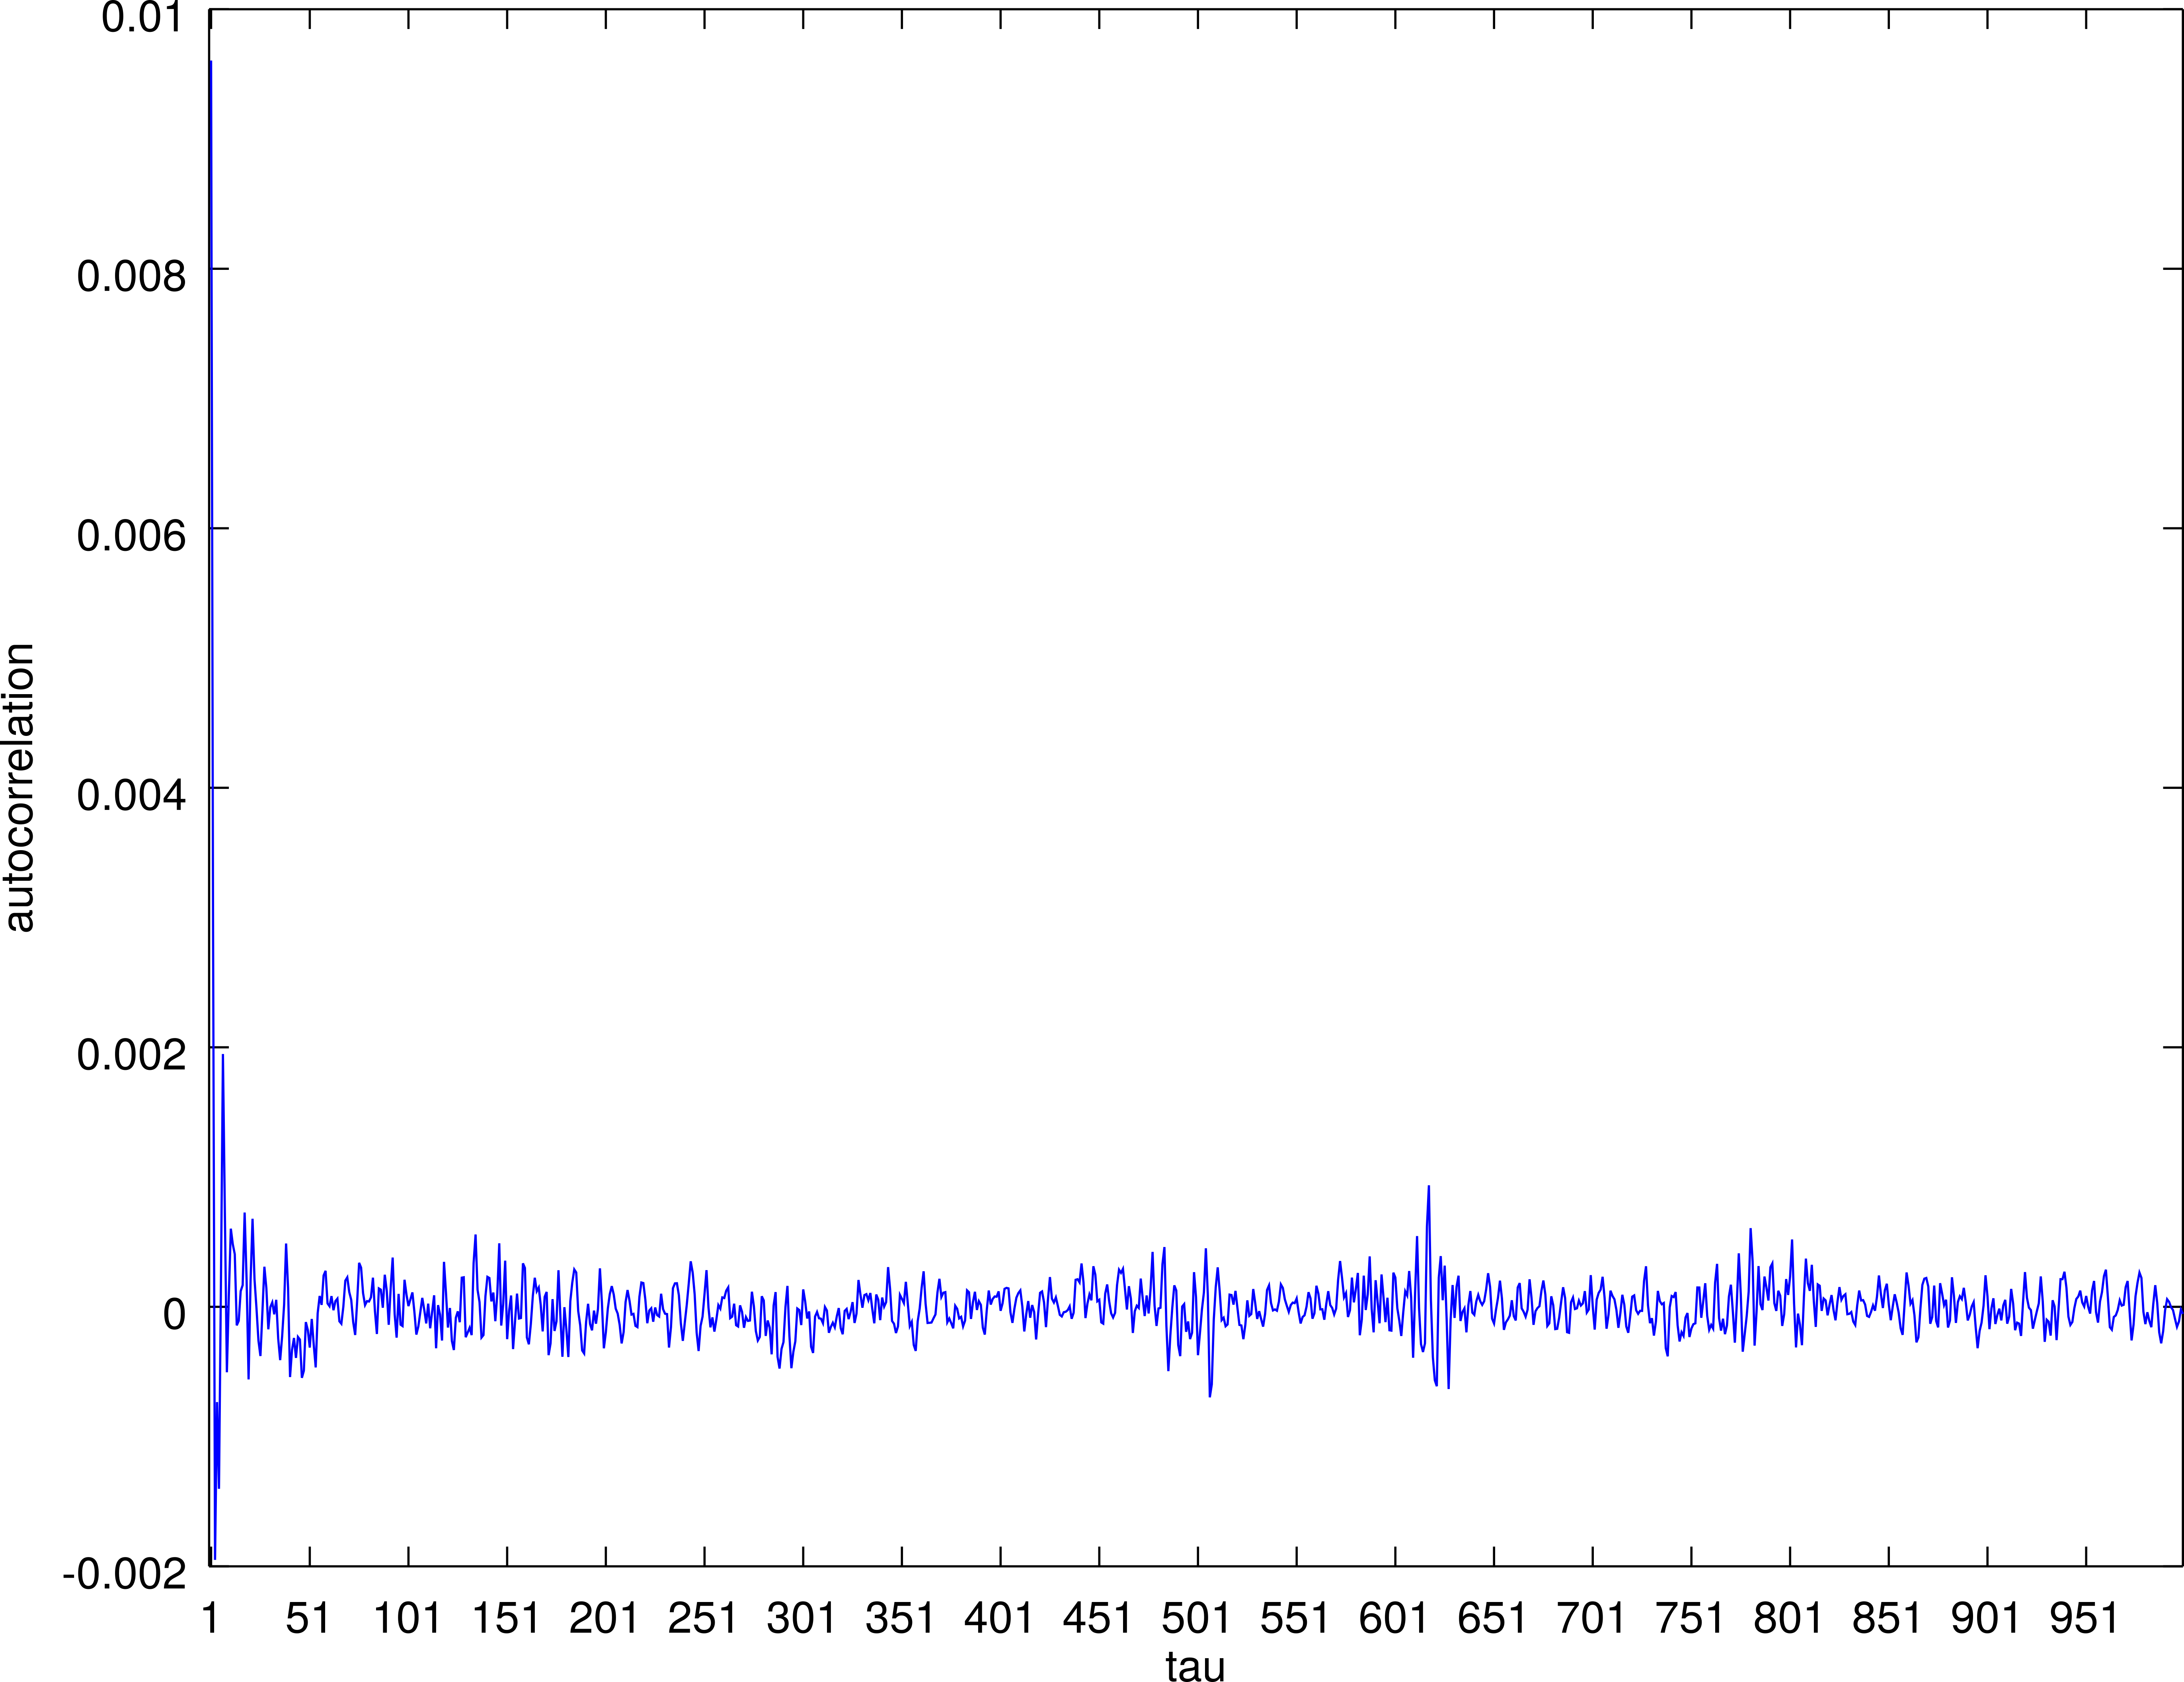
\includegraphics[width=\textheight/2]{images/cor_8.png}
         \caption{Correlation of 8' signal}
      \end{figure}
      \begin{figure}[H]
         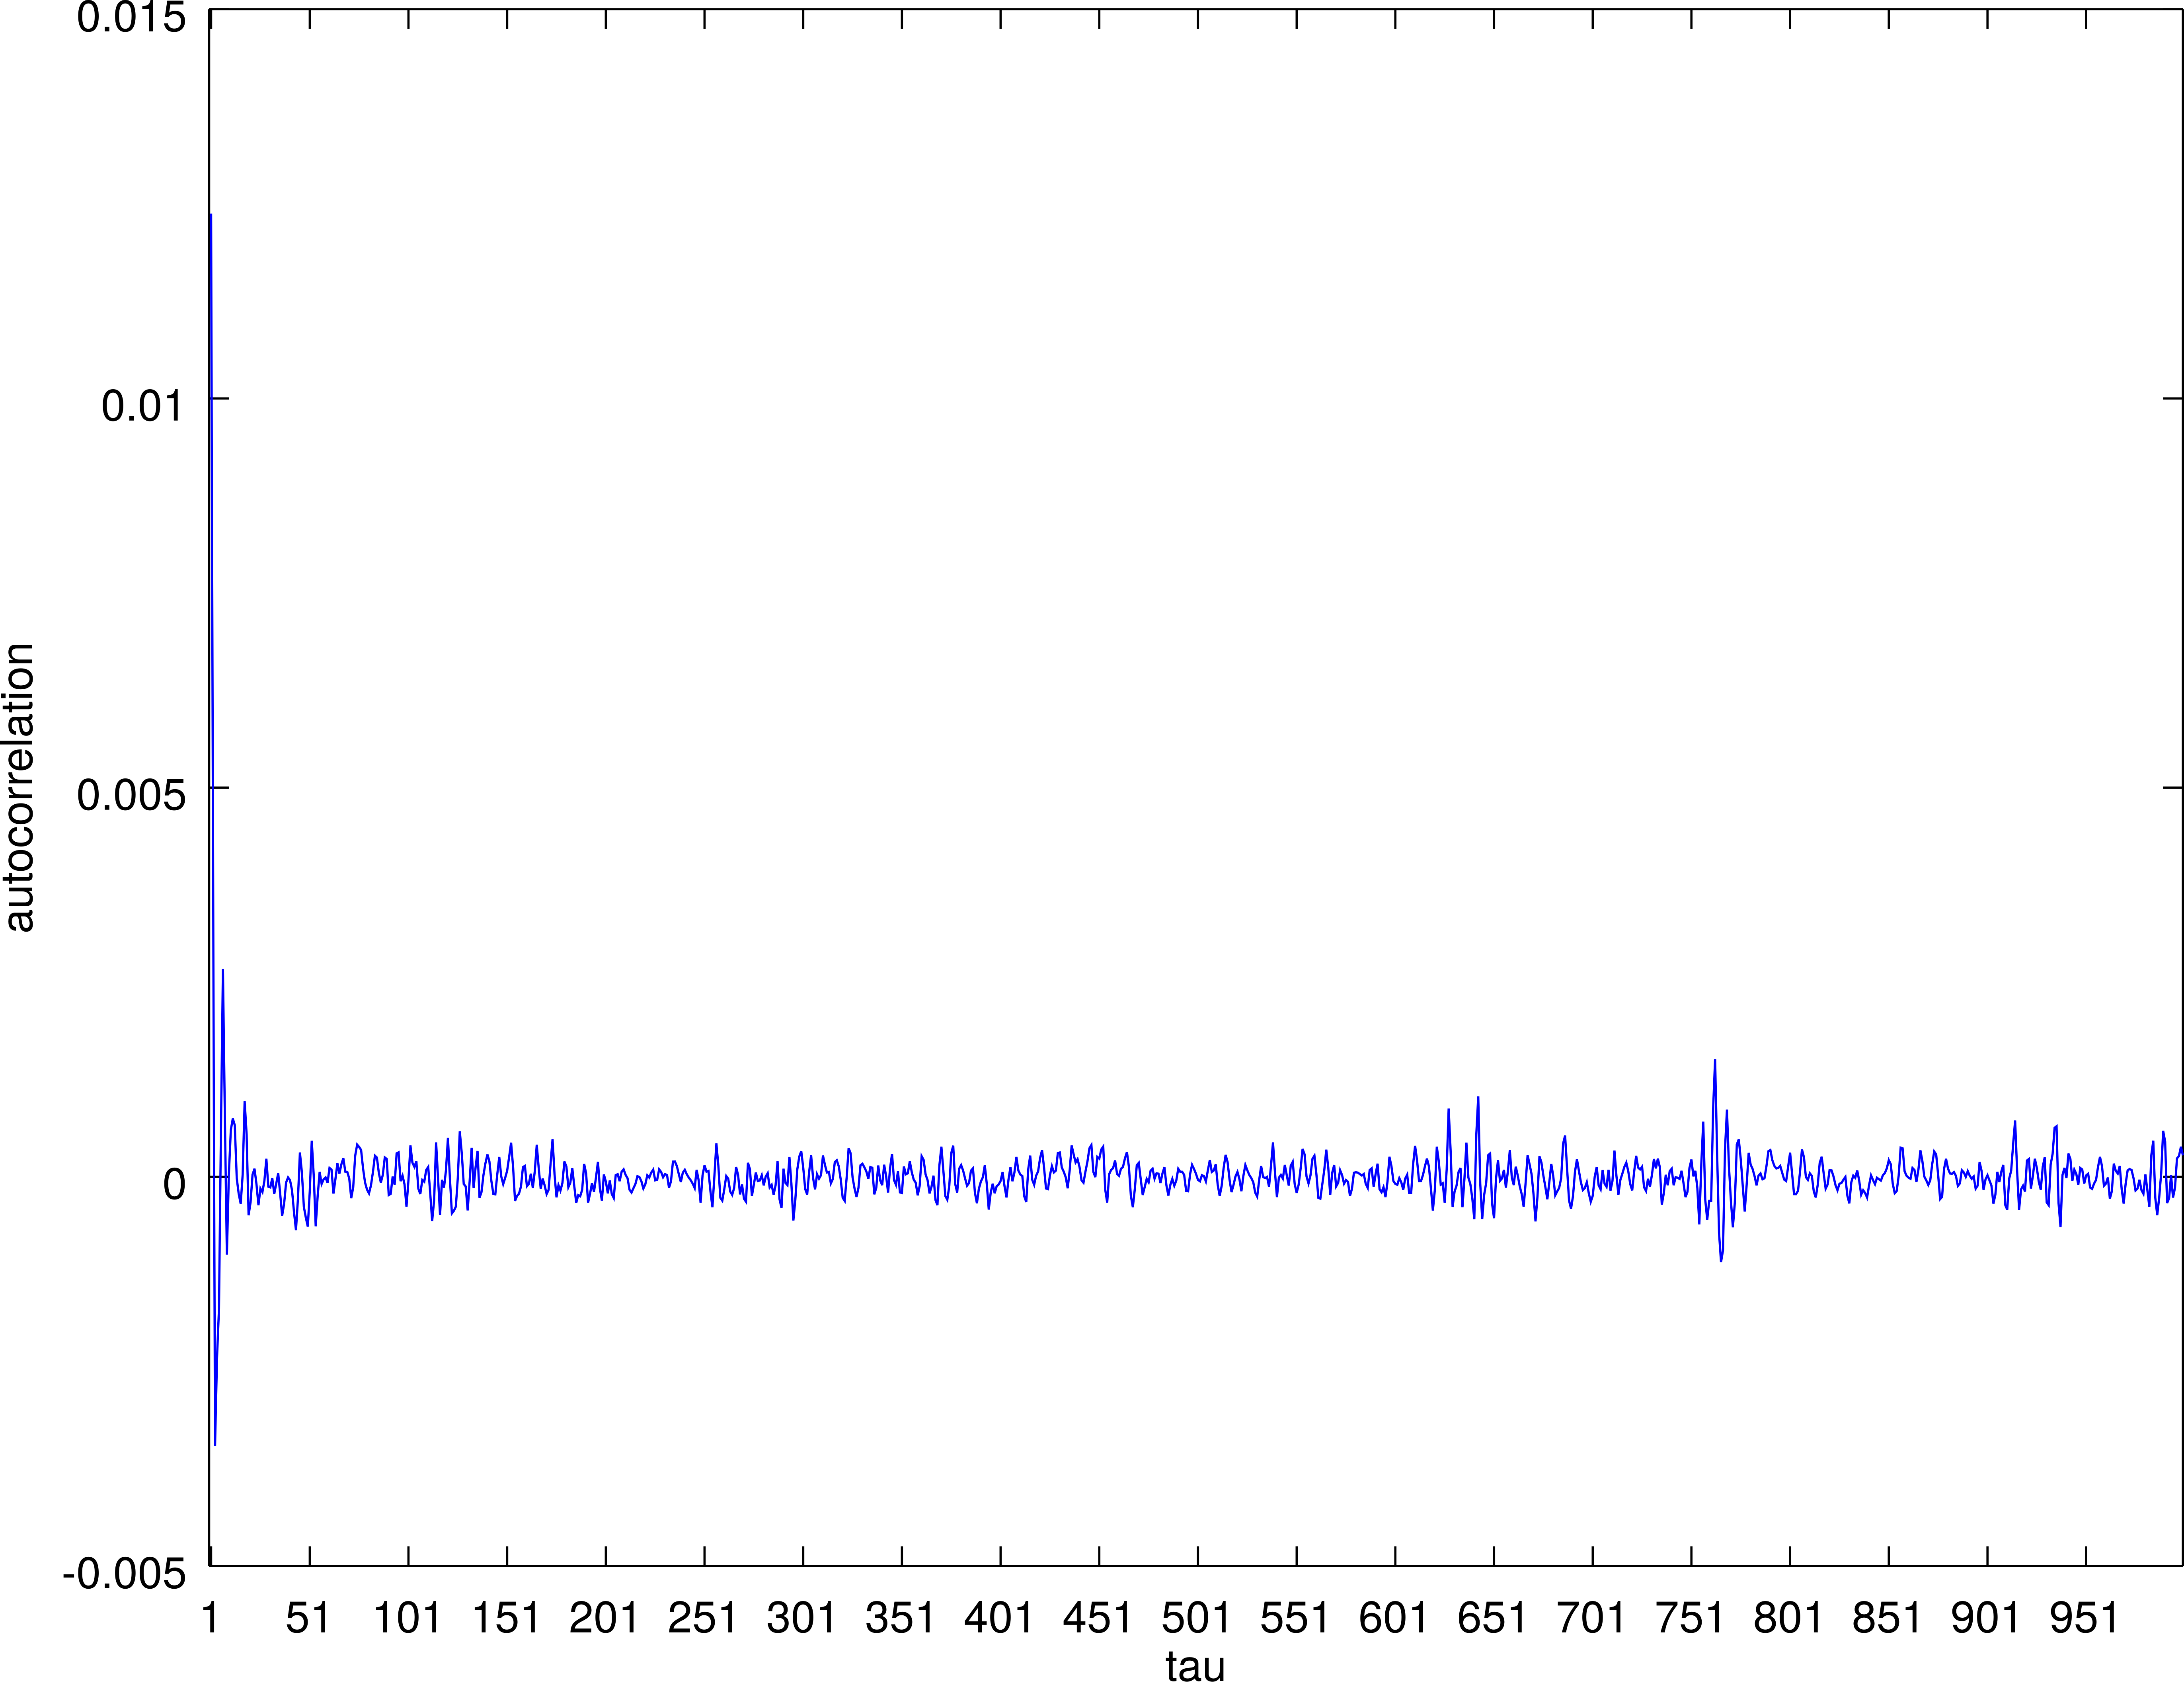
\includegraphics[width=\textheight/2]{images/cor_9.png}
         \caption{Correlation of 9'9" signal}
      \end{figure}
      \begin{figure}[H]
         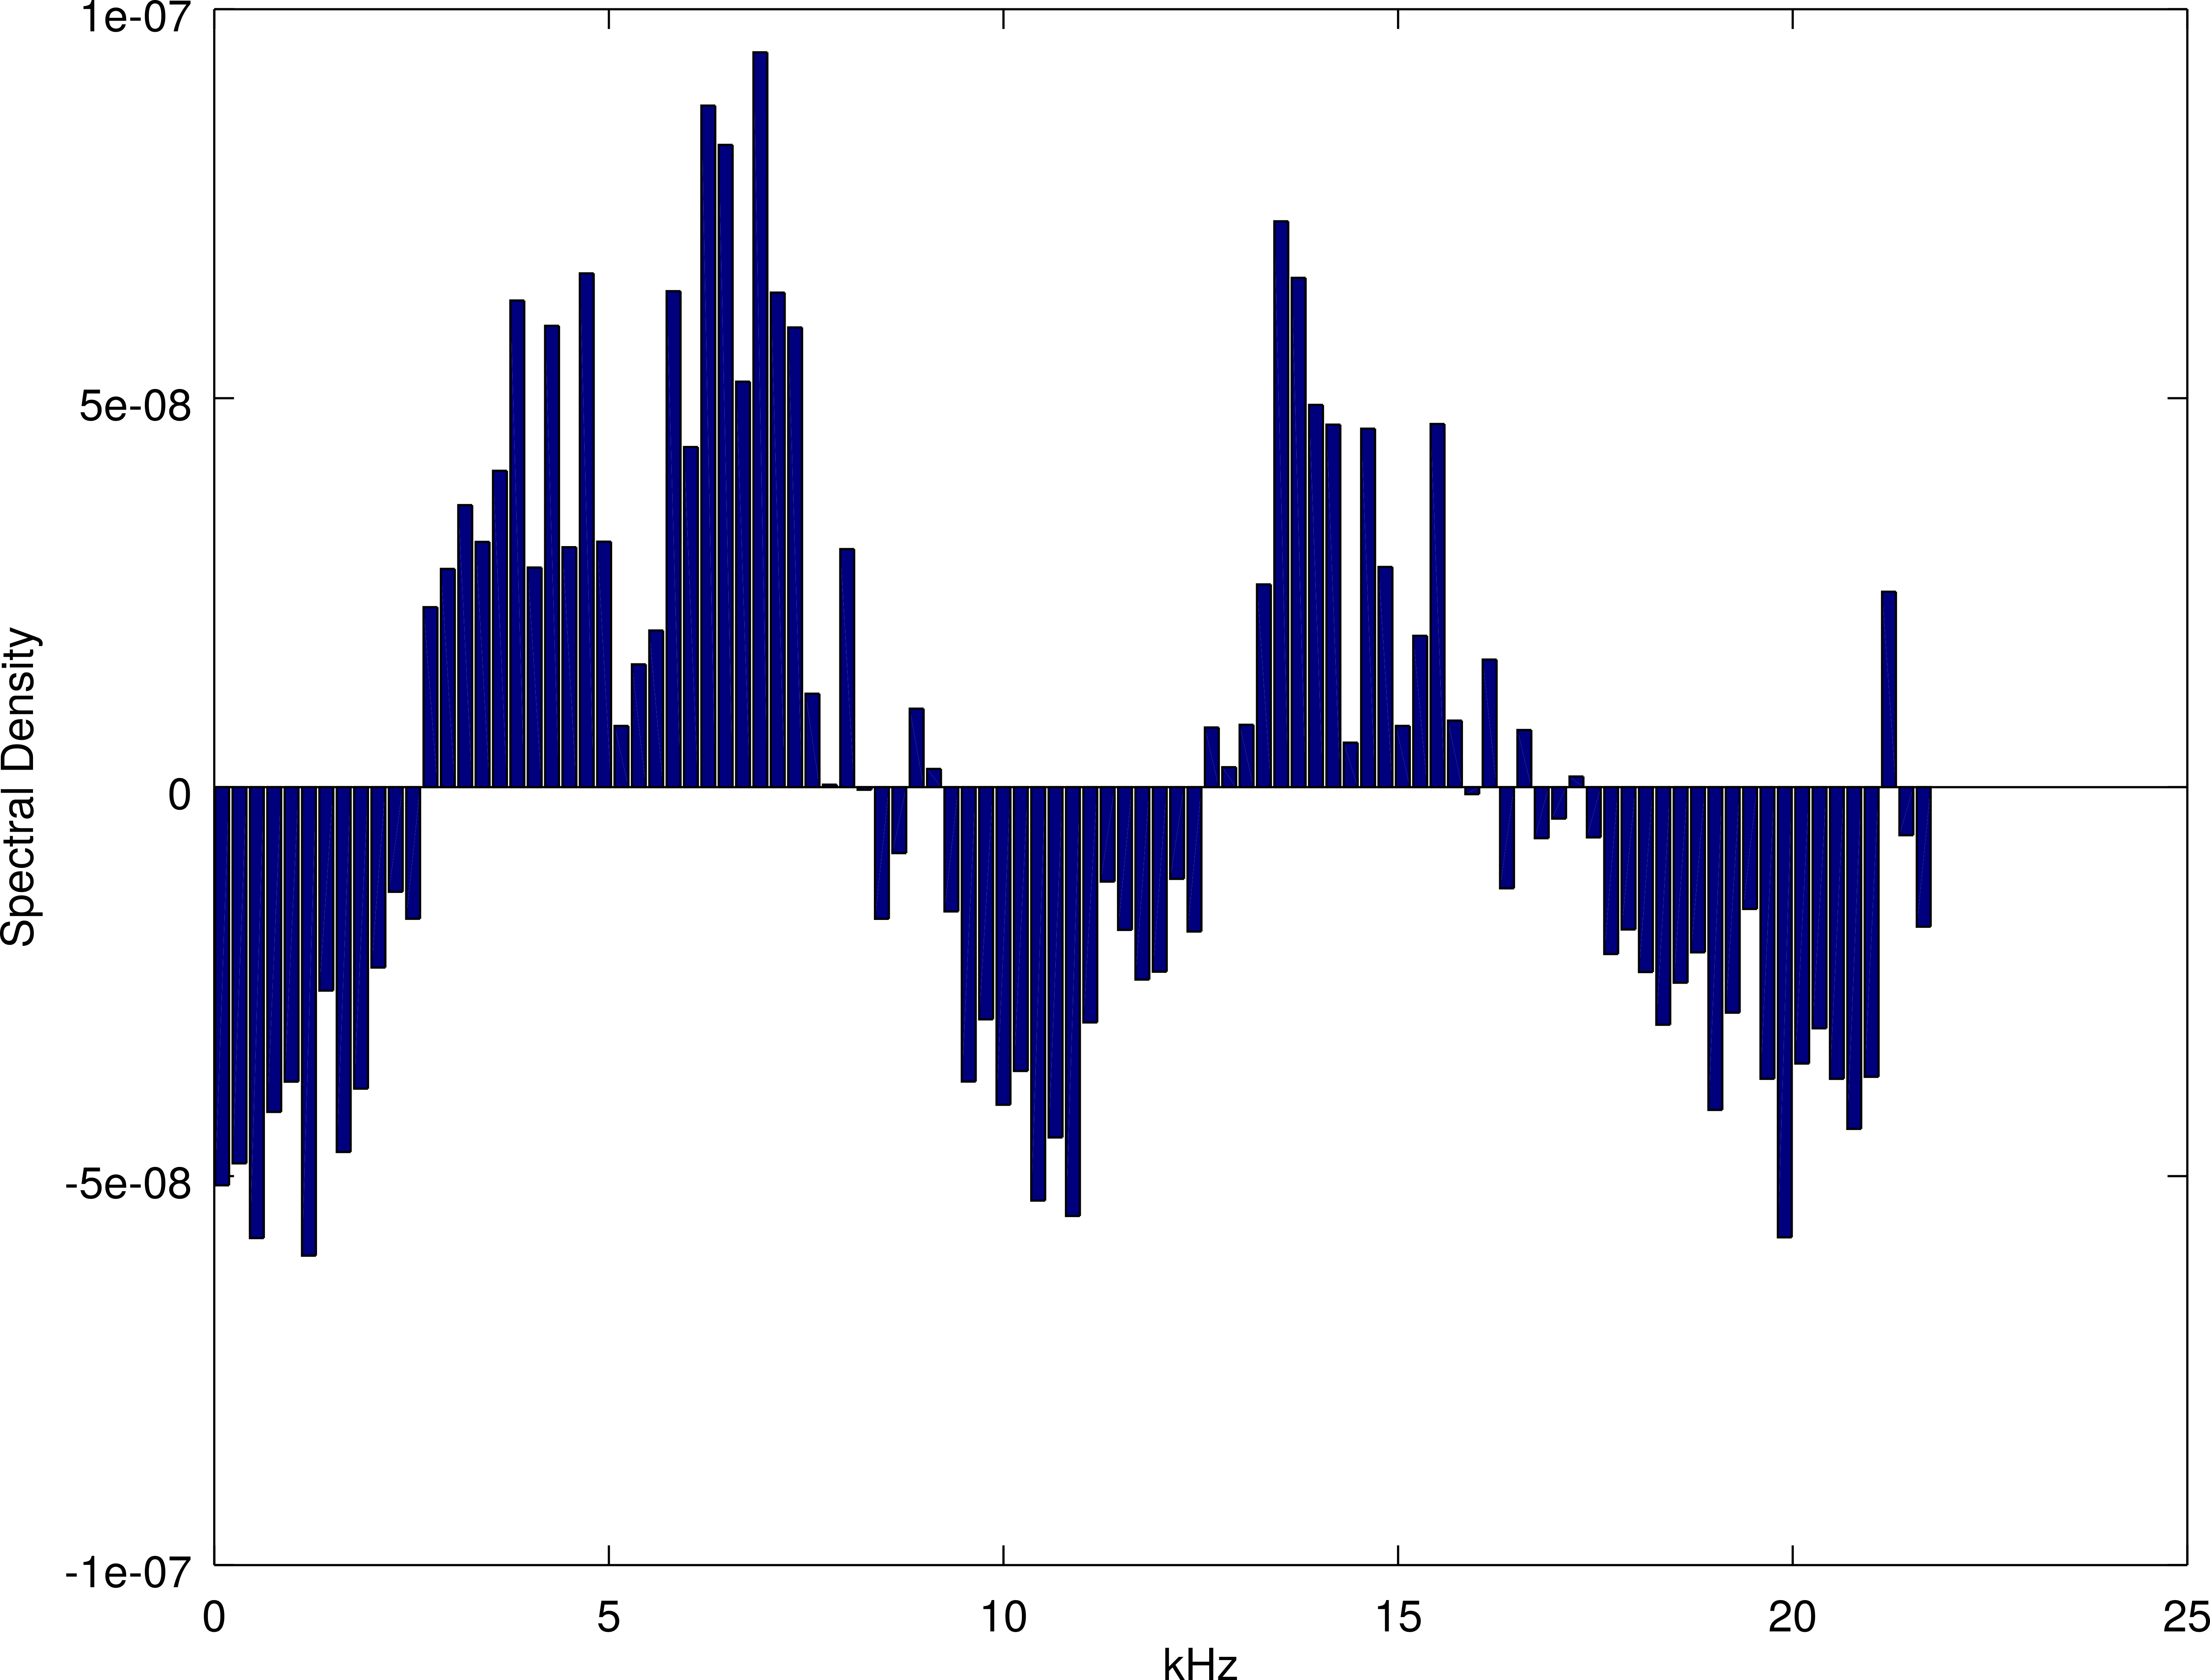
\includegraphics[width=\textheight/2]{images/spec_8.png}
         \caption{Mean subtracted Spectogram of 8' signal}
      \end{figure}
      \begin{figure}[H]
         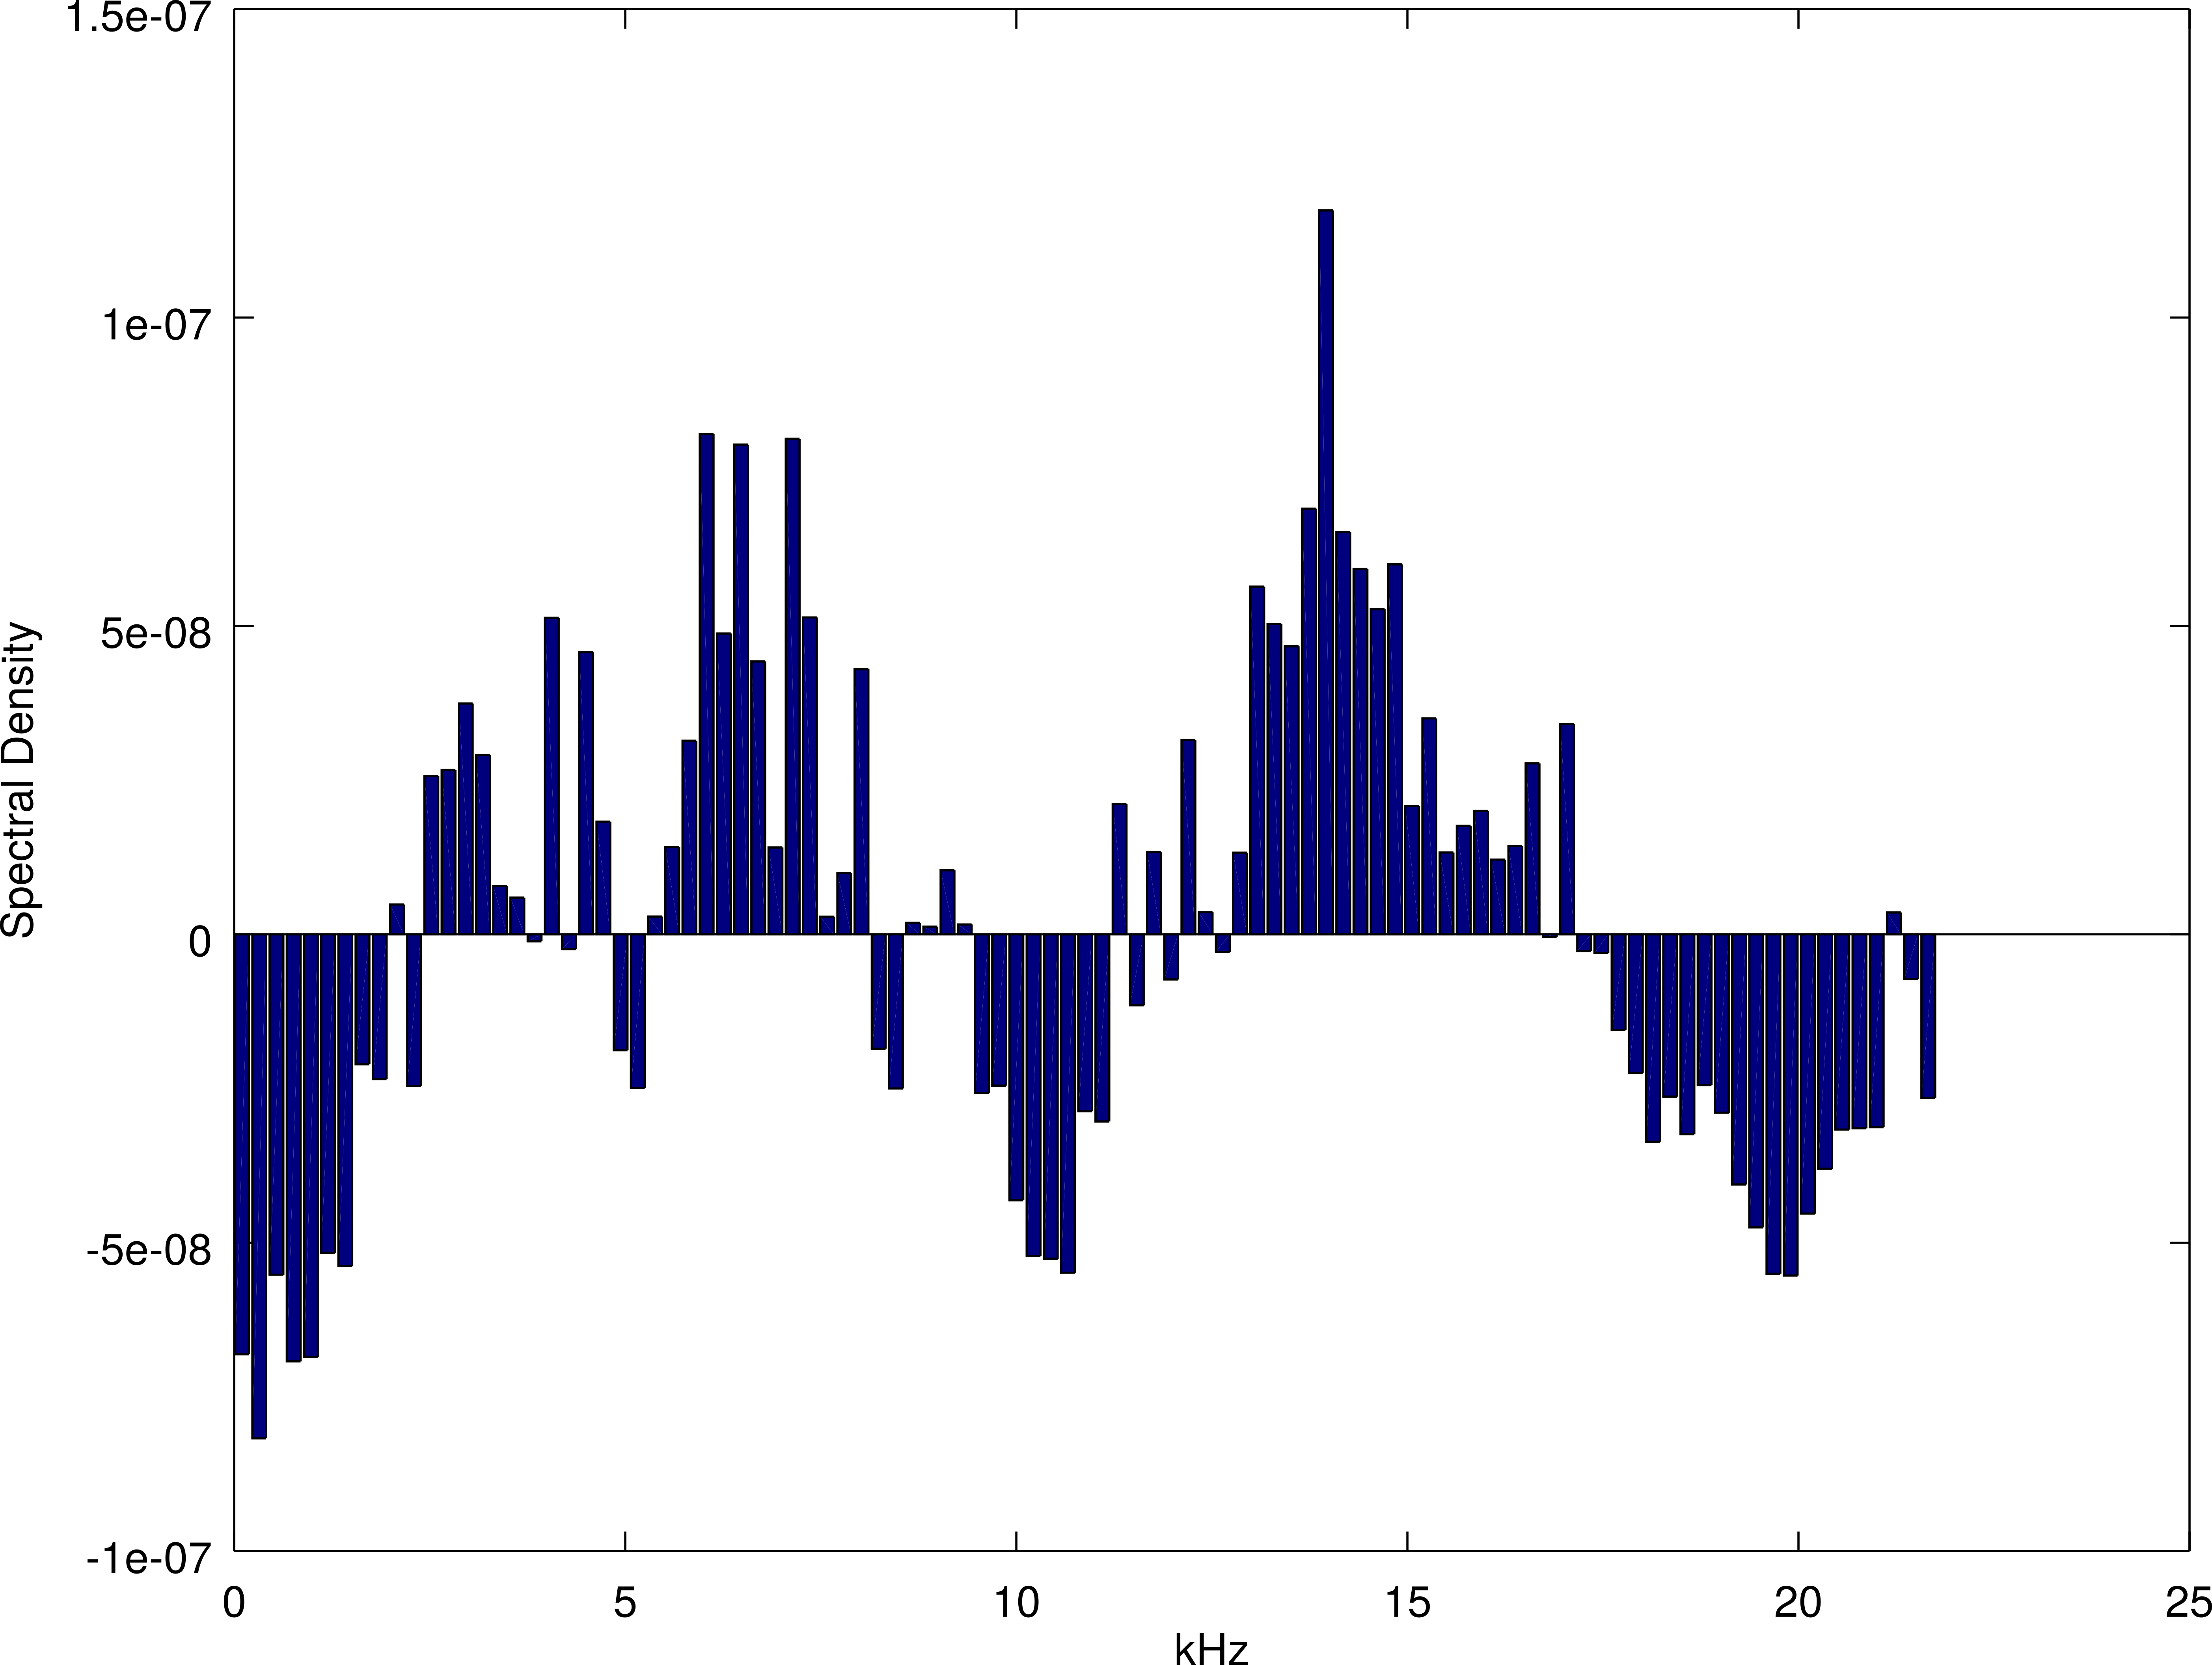
\includegraphics[width=\textheight/2]{images/spec_9.png}
         \caption{Mean subtracted Spectogram of 9'9" signal}
      \end{figure}
      Picture above is the result of running the Matlab code.
      As noticeable their is an echo in the autocorrelation of both signals
      at {620,762} for the {8', 9'9"} signal respectively. These
      numbers were approximated from their respective graphs. Computing the
      distance as described earlier yields the following information:

      \begin{tabular}{|c|c|c|}
         \hline
         Signal & Approximately Max Correlation & Theoretical Distance \\
         \hline
         8' & 620 (tau) & 7.93'\\
         9'9" & 762 (tau) & 9.74' = 9'8.9"\\
         \hline
      \end{tabular}

      Thus compared to the orginal distances, the calculated distance differed
      only by less than 1\% for both signals, using the midpoint method. Thus
      the method by which we measured the distance to the wall is an accurate
      method for the setup we had. It is noticeable that their is some blips
      in both signals except they are not the size of the main blip. Also, we
      assumed the distance of the signal to consider. This is not unreasonable
      since it may be assumed that you can guess two wide bounds to search
      between. For example, a submarine may only want to know the objects within
      100 meters of itself.

      For the spectrogram the mean was subtracted from both and the signal
      partitioned. This was to normalize and smooth the signal in the case
      of the partition. In the case of the subtracted mean, this was to
      determine if the signal was attentuated or accentuated. Examining the
      graphs above shows that in both cases the bass and mid-bass (0 - 2.5 kHz)
      was attentuated. The mids (2.5 - 9 kHz) was emphasized with a neutral zone
      The only neutral zones are around the transition points except in the
      mid zone and the low high-mids. This shows that the room was not
      neutral in terms of frequency response.
      around 5 kHz. The same procedure can be done for the high-mids and highs. 

   \section{Conclusion}
      Thus from the experiment we have determined that white noise is
      potential signal to use for the use of distance measurement. This
      signal lead to an accurate measurement within 1\% of error. Secondly,
      we showed the overall room response was tanted. The only neutral tones
      was in small areas of the frequency band. It was interesting that the
      frequency response followed a cosine wave pattern. Overall, the use of
      band-limited white noise was a success in two diverse areas of
      signal analysis.
\end{document}
